\section {Comparison to other DVCS}

There are several more distributed version control systems
we are going to explain some differences to git.
Some are:

  \begin{enumerate}
     \item \emph{Bazaar}. Powered by Cannocial. Handles the whole Ubuntu source
     repository at launchpad.net
     \item \emph{Mercurial} An opensource project initiated by Matt Mackall
     \item \emph{Perforce}. Powered by Perforce Software Inc.
     \item \emph{Visual SourceSafe} Powered by Microsoft
  \end{enumerate}
  
We are going to take a closer look at \emph{Baazar} and \emph{Mercurial} 
compared to Git.

\subsection {Data storage}

As already mentioned Git uses it's unique storage model creating new snapshots
every commit. Mercrial also thinks of its data as a snapshot. The difference
is though, that basically Mercurial also creates deltas from a revsion A to B.
Those deltas are infact the difference between two revsions. When a cumulative
amount of deltas is stored to a file, Mercurial creates a new snapshot of this file. 
\footnote{\cite {hgbook2009}
http://hgbook.red-bean.com/read/behind-the-scenes.html, section Fast retrieval,
accessed on 14.11.2010}
Baazar plans to change its model and use socalled \emph{nested trees}. At the level of data storage they are quite similar to git. The difference is that nested trees use unversioned branch data to store data instead of version files. \footnote{ http://wiki.bazaar.canonical.com/NestedTreesDesign\#git-submodules on 21.11.2010 } Baazar ist no well documented, in fact there are very good tutorials how to use Baazar. But when it comes to technical details, there is not much official documentation.

\subsection {Speed and size}

Git claims to be a very efficient system. To mesure that there are several
methods. The website \emph{whygitisbetterthanx.com} did a quite good job to
summarize why git does handle things quite fast.
Some of these tests are very biased and it seems obvious that the author's favourite system is git. 
But there are three tests\footnote{http://doc.bazaar.canonical.com/migration/en/why-switch-to-bazaar.html\#high-storage-efficiency-and-speed on 21.11.2010} on the Baazar homepage that show that git clearly wins 
calculationg the differences from revision A to B, commiting and using the log command:

\begin{figure}[h]
  \centering
  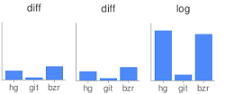
\includegraphics{img/speed.png}
  \caption{Speed tests}
  \label{fig:Speedtests}  
\end{figure}

This is the mesured time\footnote{http://doc.bazaar.canonical.com/migration/en/why-switch-to-bazaar.html\#high-storage-efficiency-and-speed on 21.11.2010}:\\

\begin{tabular}{ l || l | l | l }
Operation &	Mercurial &	Git & Bazaar \\
\hline
diff & 0.622s & 0.156s & 0.916s\\
commit & 1.126s & 0.348s & 1.030s\\
log & 3.449s & 0.402s & 3.205s\\
\end{tabular}\\

Considering size of the metadata created from the DVCS there are other several tests. Here is another one from the Baazar homepage:

\emph{The picture shows how much space the imported Mozilla project Firefox 3.5 has in the three different version control systems. The following table lists how much MB each of them needed}
\begin{figure}[h]
  \centering
  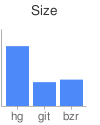
\includegraphics{img/size.png}
  \caption{Size of imported Mozilla project}
  \label{fig: The imported Mozilla project in Mercurial, Baazar and Git}  
\end{figure}

\begin{center}
\begin{tabular}{ l | c | r }
Mercurial &	Git & Bazaar \\
\hline
311M & 124M & 137M
\end{tabular}
\end{center}


